% Work-MAT -- 2. rocnik, hodina 10. Transformace mocninnych grafu, motivace exponencialy.
\documentclass[11pt,a4paper]{article}
\input{../../sablony/pripravy/priprava.sty}
\usepackage{tikz}
\usetikzlibrary{arrows.meta}
\nastavPripravu{2. ročník}{Mocninné funkce}{10}{Mocninné funkce III: transformace}
\begin{document}
\poznamka{Po testu T1 pokračujeme s mocninnými funkcemi: porovnání, posuny a jednoduché násobení předpisu konstantou. Orientačně 5 min připomenutí, 14 min transformace paraboly, 10 min posunutí hyperboly, 11 min samostatná práce, 5 min motivace exponenciální funkce. Rozšíření je rezerva.}

\blok{Jak z předpisu číst posunutí grafu?}
Známé grafy $y=x^2$ a $y=1/x$ nemusíme vždy kreslit od začátku. Změny ve vzorci umožňují předem určit jejich polohu a důležité body či asymptoty.

\begin{zadaniBox}[title={Věta - Posuny grafu funkce}]
Je-li $g(x)=f(x-a)+b$, vznikne graf $g$ z grafu $f$ posunutím o $a$ jednotek vodorovně (kladné $a$ doprava) a o $b$ jednotek svisle (kladné $b$ nahoru). Definiční obor se posune zároveň s grafem.
\end{zadaniBox}
\noindent\textbf{Zdůvodnění.}\enspace Bodu $[u;f(u)]$ původního grafu odpovídá bod $[u+a;f(u)+b]$ nového grafu. Dosazením $x=u+a$ dostaneme $g(x)=f((u+a)-a)+b=f(u)+b$.


\begin{prikladReseniBox}[title={Příklad 1}]
Z grafu $f(x)=x^2$ odvoď vlastnosti funkce $g(x)=(x-2)^2+1$. Urči vrchol, $D(g)$, $H(g)$ a nulové body.
\tcblower
Graf paraboly se posune o dvě jednotky doprava a jednu nahoru. Vrchol je $V=[2;1]$, $D(g)=\mathbb R$, $H(g)=\langle1;+\infty)$. Nulové body nejsou, protože $(x-2)^2+1\ge1$.
\end{prikladReseniBox}

\begin{center}
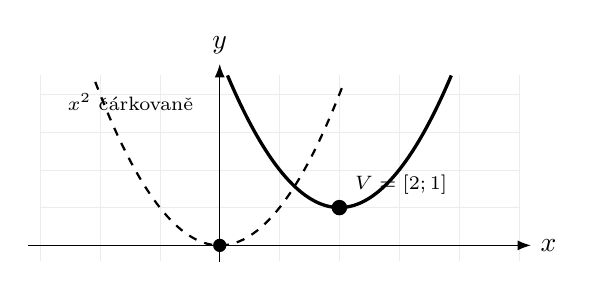
\begin{tikzpicture}[x=.76cm,y=.48cm,>=Latex]
\draw[step=1,gray!15,very thin](-3,-.4)grid(5,4.5);
\draw[->](-3.2,0)--(5.2,0)node[right]{$x$};\draw[->](0,-.45)--(0,4.8)node[above]{$y$};
\draw[dashed,thick,domain=-2.08:2.08,samples=70]plot(\x,{\x*\x});
\draw[very thick,domain=.13:3.87,samples=70]plot(\x,{(\x-2)*(\x-2)+1});
\fill(0,0)circle(2.4pt)(2,1)circle(2.8pt);
\node[font=\scriptsize,anchor=south west]at(2.1,1.1){$V=[2;1]$};
\node[font=\scriptsize,anchor=west]at(-2.7,3.8){$x^2$ čárkovaně};
\end{tikzpicture}
\end{center}
\poznamka{Kontrastuj posuny $f(x-2)$ a $f(x)+2$: první posouvá doprava, druhý nahoru. Nezaměnit rovněž inverzi $f^{-1}$ a převrácenou funkční hodnotu $1/f$.}

\blok{Posunutá hyperbola a její asymptoty}
\begin{prikladReseniBox}[title={Příklad 2}]
Je dána funkce $h(x)=\frac{1}{x-2}+1$. Urči $D(h)$, $H(h)$, asymptoty, průsečíky s osami a polohu grafu vůči $y=1/x$.
\tcblower
Graf $y=1/x$ je posunut o dvě jednotky doprava a jednu nahoru. Proto $D(h)=\mathbb R\setminus\{2\}$, $H(h)=\mathbb R\setminus\{1\}$, asymptoty $x=2$ a $y=1$. S osou $y$: $h(0)=\frac12$, tedy bod $[0;1/2]$. S osou $x$: $\frac1{x-2}+1=0$, odkud $x=1$, tedy $[1;0]$.
\end{prikladReseniBox}

\begin{prikladReseniBox}[title={Příklad 3}]
Jak se změní graf funkce $f(x)=x^3$, jestliže přejdeme k $g(x)=-2x^3$?
\tcblower
Násobení hodnot číslem $-2$ znamená osovou souměrnost podle osy $x$ a dvojnásobné svislé protažení. Funkce $g$ je stále lichá, má $D(g)=H(g)=\mathbb R$, ale je přísně klesající.
\end{prikladReseniBox}

\blok{Samostatná práce}
\begin{zadaniReseniBox}[title={Samostatná práce 1}]
\begin{enumerate}[label=\alph*)]
\item U $f(x)=(x+1)^2-4$ urči vrchol, $H(f)$ a nulové body.
\item U $g(x)=\frac2{x+3}-2$ urči $D(g)$, $H(g)$ a obě asymptoty.
\item Popiš, jak vznikne graf $h(x)=-x^4$ z grafu $y=x^4$. Urči $H(h)$.
\end{enumerate}
\tcblower
\begin{enumerate}[label=\alph*)]
\item Vrchol $[-1;-4]$, $H(f)=\langle-4;+\infty)$, nulové body $x=-3$ a $x=1$.
\item $D(g)=\mathbb R\setminus\{-3\}$, $H(g)=\mathbb R\setminus\{-2\}$, asymptoty $x=-3$ a $y=-2$.
\item Graf je převrácen souměrností podle osy $x$. $H(h)=(-\infty;0\rangle$.
\end{enumerate}
\end{zadaniReseniBox}

\begin{zadaniReseniBox}[title={Rozšíření 1}]
Pro $p(x)=-\frac{2}{(x-1)^2}+3$ urči definiční obor, obor hodnot, asymptoty a nejvyšší možnou horní mez $3$ (zda se dosahuje).
\tcblower
$D(p)=\mathbb R\setminus\{1\}$, $H(p)=(-\infty;3)$. Asymptoty jsou $x=1$, $y=3$. Číslo $3$ je horní mezí a supremem oboru hodnot, ale není funkční hodnotou, takže maximum neexistuje.
\end{zadaniReseniBox}

\blok{Most k hodině 11: proměnný exponent}
U mocninné funkce $x^n$ je \textbf{základ proměnný} a exponent je pevný. Příště budeme zkoumat opačný typ předpisu: $a^x$, kde je \textbf{základ pevný} a proměnná je v exponentu. Například $x^2$ a $2^x$ dávají pro $x=0$ hodnoty $0$ a $1$, pro $x=1$ hodnoty $1$ a $2$ a pro $x=2$ obě hodnotu $4$. Z těchto několika bodů ovšem nemůžeme usuzovat na stejný průběh grafů.

\begin{zadaniReseniBox}[title={Domácí úkol}]
\begin{enumerate}[label=\alph*)]
\item Urči vrchol a obor hodnot $f(x)=(x-3)^2+2$.
\item Urči asymptoty $g(x)=\frac{4}{x+1}-3$ a vypočítej $g(0)$.
\item Doplň hodnoty $x^2$ a $2^x$ pro $x=0,1,2,3$.
\end{enumerate}
\tcblower
\begin{enumerate}[label=\alph*)]
\item Vrchol $[3;2]$, $H(f)=\langle2;+\infty)$.
\item Asymptoty $x=-1$ a $y=-3$; $g(0)=1$.
\item $x^2$: $0,1,4,9$; $2^x$: $1,2,4,8$.
\end{enumerate}
\end{zadaniReseniBox}
\end{document}
